\documentclass[12pt,letterpaper]{article}
\usepackage{graphicx,textcomp}
\usepackage{natbib}
\usepackage{setspace}
\usepackage{fullpage}
\usepackage{color}
\usepackage[reqno]{amsmath}
\usepackage{amsthm}
\usepackage{fancyvrb}
\usepackage{amssymb,enumerate}
\usepackage[all]{xy}
\usepackage{endnotes}
\usepackage{lscape}
\newtheorem{com}{Comment}
\usepackage{float}
\usepackage{hyperref}
\newtheorem{lem} {Lemma}
\newtheorem{prop}{Proposition}
\newtheorem{thm}{Theorem}
\newtheorem{defn}{Definition}
\newtheorem{cor}{Corollary}
\newtheorem{obs}{Observation}
\usepackage[compact]{titlesec}
\usepackage{dcolumn}
\usepackage{tikz}
\usetikzlibrary{arrows}
\usepackage{multirow}
\usepackage{xcolor}
\newcolumntype{.}{D{.}{.}{-1}}
\newcolumntype{d}[1]{D{.}{.}{#1}}
\definecolor{light-gray}{gray}{0.65}
\usepackage{url}
\usepackage{listings}
\usepackage{color}

\definecolor{codegreen}{rgb}{0,0.6,0}
\definecolor{codegray}{rgb}{0.5,0.5,0.5}
\definecolor{codepurple}{rgb}{0.58,0,0.82}
\definecolor{backcolour}{rgb}{0.95,0.95,0.92}

\lstdefinestyle{mystyle}{
	backgroundcolor=\color{backcolour},   
	commentstyle=\color{codegreen},
	keywordstyle=\color{magenta},
	numberstyle=\tiny\color{codegray},
	stringstyle=\color{codepurple},
	basicstyle=\footnotesize,
	breakatwhitespace=false,         
	breaklines=true,                 
	captionpos=b,                    
	keepspaces=true,                 
	numbers=left,                    
	numbersep=5pt,                  
	showspaces=false,                
	showstringspaces=false,
	showtabs=false,                  
	tabsize=2
}
\lstset{style=mystyle}
\newcommand{\Sref}[1]{Section~\ref{#1}}
\newtheorem{hyp}{Hypothesis}

\title{Problem Set 3}
\date{Due: November 20, 2021}
\author{Applied Stats/Quant Methods 1}


\begin{document}
	\maketitle
	\section*{Instructions}
	\begin{itemize}
		\item Please show your work! You may lose points by simply writing in the answer. If the problem requires you to execute commands in \texttt{R}, please include the code you used to get your answers. Please also include the \texttt{.R} file that contains your code. If you are not sure if work needs to be shown for a particular problem, please ask.
	\item Your homework should be submitted electronically on GitHub.
	\item This problem set is due before 23:59 on Sunday November 20, 2022. No late assignments will be accepted.
	\item Total available points for this homework is 80.
	\end{itemize}

		\vspace{.25cm}
	
\noindent In this problem set, you will run several regressions and create an add variable plot (see the lecture slides) in \texttt{R} using the \texttt{incumbents\_subset.csv} dataset. Include all of your code.

\newpage

\section*{Question 1}
\vspace{.25cm}
\noindent We are interested in knowing how the difference in campaign spending between incumbent and challenger affects the incumbent's vote share.

\begin{enumerate}
	\item \textbf{Run a regression where the outcome variable is \texttt{voteshare} and the explanatory variable is \texttt{difflog}.}
		
		\lstinputlisting[language=R, firstline=21, lastline=22]{PS03_answersLucasDeMeloPrado.R}		
		
		\begin{table}[H] \centering 
			\caption{The association between \texttt{difflog} and \texttt{voteshare}} 
			\label{} 
			\begin{tabular}{@{\extracolsep{5pt}}lc} 
				\\[-1.8ex]\hline 
				\hline \\[-1.8ex] 
				& \multicolumn{1}{c}{\textit{Dependent variable:}} \\ 
				\cline{2-2} 
				\\[-1.8ex] & \texttt{voteshare} \\ 
				\hline \\[-1.8ex] 
				\texttt{difflog} & 0.042$^{***}$ \\ 
				& (0.001) \\ 
				& \\ 
				Constant & 0.579$^{***}$ \\ 
				& (0.002) \\ 
				& \\ 
				\hline \\[-1.8ex] 
				Observations & 3,193 \\ 
				R$^{2}$ & 0.367 \\ 
				Adjusted R$^{2}$ & 0.367 \\ 
				Residual Std. Error & 0.079 (df = 3191) \\ 
				F Statistic & 1,852.791$^{***}$ (df = 1; 3191) \\ 
				\hline 
				\hline \\[-1.8ex] 
				\textit{Note:}  & \multicolumn{1}{r}{$^{*}$p$<$0.1; $^{**}$p$<$0.05; $^{***}$p$<$0.01} \\ 
			\end{tabular} 
		\end{table} 
		
	\item \textbf{Make a scatterplot of the two variables and add the regression line.}

		\lstinputlisting[language=R, firstline=25, lastline=31]{PS03_answersLucasDeMeloPrado.R}
		
		\begin{figure}[H]
			\centering
			\caption{The association between \texttt{difflog} and \texttt{voteshare}}
			\label{fig:lm_q1}
			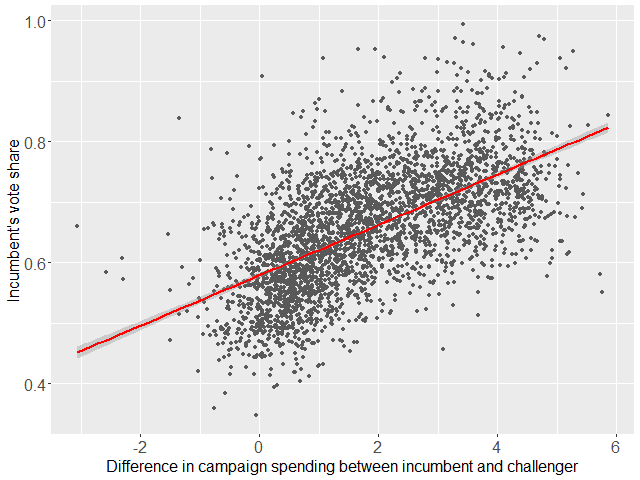
\includegraphics[width=0.9\linewidth]{lm_q1}
		\end{figure}

	\item \textbf{Save the residuals of the model in a separate object.}

		\lstinputlisting[language=R, firstline=34, lastline=34]{PS03_answersLucasDeMeloPrado.R}

	\item \textbf{Write the prediction equation.}
	\end{enumerate}
	
		$$y = \beta_0 + \beta_1 x$$
		$$y = 0.579 + 0.042x$$
	
\newpage

\section*{Question 2}
\noindent We are interested in knowing how the difference between incumbent and challenger's spending and the vote share of the presidential candidate of the incumbent's party are related.

\begin{enumerate}
	\item \textbf{Run a regression where the outcome variable is \texttt{presvote} and the explanatory variable is \texttt{difflog}.}

		\lstinputlisting[language=R, firstline=41, lastline=42]{PS03_answersLucasDeMeloPrado.R}

		\begin{table}[H] \centering 
			\caption{The association between \texttt{difflog} and \texttt{presvote}} 
			\label{} 
			\begin{tabular}{@{\extracolsep{5pt}}lc} 
				\\[-1.8ex]\hline 
				\hline \\[-1.8ex] 
				& \multicolumn{1}{c}{\textit{Dependent variable:}} \\ 
				\cline{2-2} 
				\\[-1.8ex] & \texttt{presvote} \\ 
				\hline \\[-1.8ex] 
				\texttt{difflog} & 0.024$^{***}$ \\ 
				& (0.001) \\ 
				& \\ 
				Constant & 0.508$^{***}$ \\ 
				& (0.003) \\ 
				& \\ 
				\hline \\[-1.8ex] 
				Observations & 3,193 \\ 
				R$^{2}$ & 0.088 \\ 
				Adjusted R$^{2}$ & 0.088 \\ 
				Residual Std. Error & 0.110 (df = 3191) \\ 
				F Statistic & 307.715$^{***}$ (df = 1; 3191) \\ 
				\hline 
				\hline \\[-1.8ex] 
				\textit{Note:}  & \multicolumn{1}{r}{$^{*}$p$<$0.1; $^{**}$p$<$0.05; $^{***}$p$<$0.01} \\ 
			\end{tabular} 
		\end{table} 
	
	\item \textbf{Make a scatterplot of the two variables and add the regression line.}
	
		\lstinputlisting[language=R, firstline=45, lastline=51]{PS03_answersLucasDeMeloPrado.R}

		\begin{figure}[H]
			\centering
			\caption{The association between \texttt{difflog} and \texttt{presvote}}
			\label{fig:lm_q2}
			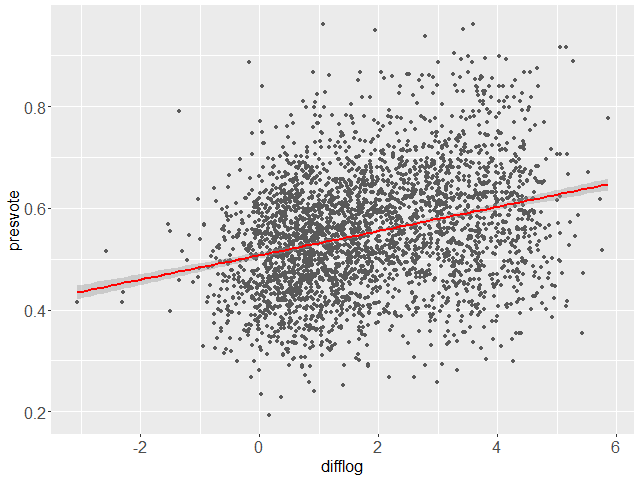
\includegraphics[width=0.9\linewidth]{lm_q2}
		\end{figure}
	
	\item \textbf{Save the residuals of the model in a separate object.}
	
		\lstinputlisting[language=R, firstline=54, lastline=54]{PS03_answersLucasDeMeloPrado.R}
	
	\item \textbf{Write the prediction equation.}
	
		$$y = \beta_0 + \beta_1 x$$
		$$y = 0.508 + 0.024x$$
		
	\end{enumerate}
	
	\newpage

\section*{Question 3}

\noindent We are interested in knowing how the vote share of the presidential candidate of the incumbent's party is associated with the incumbent's electoral success.

\begin{enumerate}
	\item \textbf{Run a regression where the outcome variable is \texttt{voteshare} and the explanatory variable is \texttt{presvote}.}

		\lstinputlisting[language=R, firstline=61, lastline=62]{PS03_answersLucasDeMeloPrado.R}

		\begin{table}[H] \centering 
			\caption{The association between \texttt{presvote} and \texttt{voteshare}} 
			\label{} 
			\begin{tabular}{@{\extracolsep{5pt}}lc} 
				\\[-1.8ex]\hline 
				\hline \\[-1.8ex] 
				& \multicolumn{1}{c}{\textit{Dependent variable:}} \\ 
				\cline{2-2} 
				\\[-1.8ex] & \texttt{voteshare} \\ 
				\hline \\[-1.8ex] 
				\texttt{presvote} & 0.388$^{***}$ \\ 
				& (0.013) \\ 
				& \\ 
				Constant & 0.441$^{***}$ \\ 
				& (0.008) \\ 
				& \\ 
				\hline \\[-1.8ex] 
				Observations & 3,193 \\ 
				R$^{2}$ & 0.206 \\ 
				Adjusted R$^{2}$ & 0.206 \\ 
				Residual Std. Error & 0.088 (df = 3191) \\ 
				F Statistic & 826.950$^{***}$ (df = 1; 3191) \\ 
				\hline 
				\hline \\[-1.8ex] 
				\textit{Note:}  & \multicolumn{1}{r}{$^{*}$p$<$0.1; $^{**}$p$<$0.05; $^{***}$p$<$0.01} \\ 
			\end{tabular} 
		\end{table} 

	\item \textbf{Make a scatterplot of the two variables and add the regression line.}

		\lstinputlisting[language=R, firstline=65, lastline=71]{PS03_answersLucasDeMeloPrado.R}

		\begin{figure}[H]
			\centering
			\caption{The association between \texttt{presvote} and \texttt{voteshare}}
			\label{fig:lm_q3}
			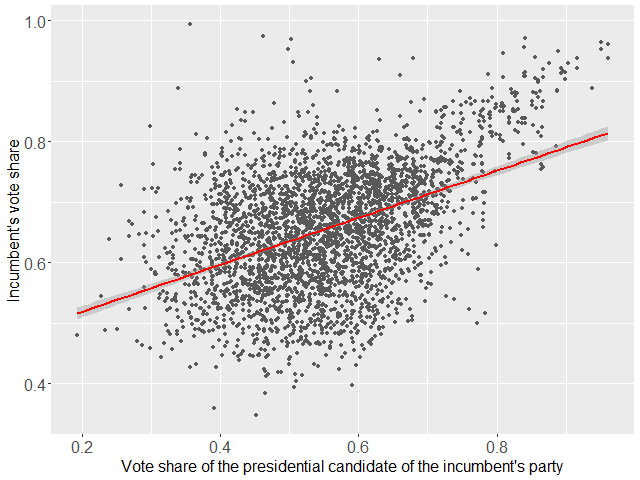
\includegraphics[width=0.9\linewidth]{lm_q3}
		\end{figure}

	\item \textbf{Write the prediction equation.}
	
		$$y = \beta_0 + \beta_1 x$$
		$$y = 0.441 + 0.388x$$
	
\end{enumerate}
	
\newpage

\section*{Question 4}
\noindent The residuals from part (a) tell us how much of the variation in \texttt{voteshare} is $not$ explained by the difference in spending between incumbent and challenger. The residuals in part (b) tell us how much of the variation in \texttt{presvote} is $not$ explained by the difference in spending between incumbent and challenger in the district.

\begin{enumerate}
	\item \textbf{Run a regression where the outcome variable is the residuals from Question 1 and the explanatory variable is the residuals from Question 2.}

		\lstinputlisting[language=R, firstline=79, lastline=83]{PS03_answersLucasDeMeloPrado.R}
		
		\begin{table}[H] \centering 
			\caption{The association between the residuals from Question 1 and Question 2} 
			\label{} 
			\begin{tabular}{@{\extracolsep{5pt}}lc} 
				\\[-1.8ex]\hline 
				\hline \\[-1.8ex] 
				& \multicolumn{1}{c}{\textit{Dependent variable:}} \\ 
				\cline{2-2} 
				\\[-1.8ex] & Residuals from Question 1 \\ 
				\hline \\[-1.8ex] 
				Residuals from Question 2 & 0.257$^{***}$ \\ 
				& (0.012) \\ 
				& \\ 
				Constant & $-$0.000 \\ 
				& (0.001) \\ 
				& \\ 
				\hline \\[-1.8ex] 
				Observations & 3,193 \\ 
				R$^{2}$ & 0.130 \\ 
				Adjusted R$^{2}$ & 0.130 \\ 
				Residual Std. Error & 0.073 (df = 3191) \\ 
				F Statistic & 476.975$^{***}$ (df = 1; 3191) \\ 
				\hline 
				\hline \\[-1.8ex] 
				\textit{Note:}  & \multicolumn{1}{r}{$^{*}$p$<$0.1; $^{**}$p$<$0.05; $^{***}$p$<$0.01} \\ 
			\end{tabular} 
		\end{table} 

	\item \textbf{Make a scatterplot of the two residuals and add the regression line.}

		\lstinputlisting[language=R, firstline=86, lastline=94]{PS03_answersLucasDeMeloPrado.R}	

		\begin{figure}[H]
			\centering
			\caption{The association between the residuals from Question 1 and Question 2}
			\label{fig:lm_q4}
			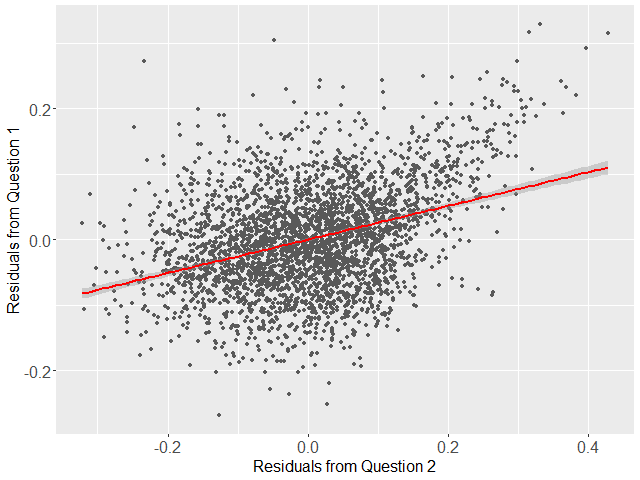
\includegraphics[width=0.9\linewidth]{lm_q4}
		\end{figure}

	\item \textbf{Write the prediction equation.}
	
		$$y = \beta_0 + \beta_1 x$$
		$$y = 0 + 0.257x$$
		$$y = 0.257x$$
	
\end{enumerate}
	
\newpage	

\section*{Question 5}
\noindent What if the incumbent's vote share is affected by both the president's popularity and the difference in spending between incumbent and challenger? 

\begin{enumerate}
	\item \textbf{Run a regression where the outcome variable is the incumbent's \texttt{voteshare} and the explanatory variables are \texttt{difflog} and \texttt{presvote}.}

		\lstinputlisting[language=R, firstline=102, lastline=103]{PS03_answersLucasDeMeloPrado.R}

		\begin{table}[!htbp] \centering 
			\caption{The association among \texttt{difflog}, \texttt{presvote}, and \texttt{voteshare}} 
			\label{} 
			\begin{tabular}{@{\extracolsep{5pt}}lccc} 
				\\[-1.8ex]\hline 
				\hline \\[-1.8ex] 
				& \multicolumn{3}{c}{\textit{Dependent variable:}} \\ 
				\cline{2-4} 
				\\[-1.8ex] & \multicolumn{3}{c}{\texttt{voteshare}} \\ 
				\\[-1.8ex] & (1) & (2) & (3)\\ 
				\hline \\[-1.8ex] 
				\texttt{difflog} & 0.042$^{***}$ &  & 0.036$^{***}$ \\ 
				& (0.001) &  & (0.001) \\ 
				& & & \\ 
				\texttt{presvote} &  & 0.388$^{***}$ & 0.257$^{***}$ \\ 
				&  & (0.013) & (0.012) \\ 
				& & & \\ 
				Constant & 0.579$^{***}$ & 0.441$^{***}$ & 0.449$^{***}$ \\ 
				& (0.002) & (0.008) & (0.006) \\ 
				& & & \\ 
				\hline \\[-1.8ex] 
				Observations & 3,193 & 3,193 & 3,193 \\ 
				R$^{2}$ & 0.367 & 0.206 & 0.450 \\ 
				Adjusted R$^{2}$ & 0.367 & 0.206 & 0.449 \\ 
				Residual Std. Error & 0.079 & 0.088 & 0.073 \\ 
				& (df = 3191) & (df = 3191) & (df = 3190) \\
				F Statistic & 1,852.791$^{***}$ & 826.950$^{***}$ & 1,302.947$^{***}$ \\ 
				& (df = 1; 3191) & (df = 1; 3191) & (df = 2; 3190) \\
				\hline 
				\hline \\[-1.8ex] 
				\textit{Note:}  & \multicolumn{3}{r}{$^{*}$p$<$0.1; $^{**}$p$<$0.05; $^{***}$p$<$0.01} \\ 
			\end{tabular} 
		\end{table} 

	\item \textbf{Write the prediction equation.}

		$$y = \beta_0 + \beta_1 x_1 + \beta_2 x_2$$
		$$y = 0.449 + 0.036x_1 + 0.257x_2$$

	\item \textbf{What is it in this output that is identical to the output in Question 4? Why do you think this is the case?}
	
		The slope ($\beta_1$) in the bivariate regression model of the residuals ($y=0.257x$) is the same slope ($\beta_2$) of the variable \texttt{presvote} ($x_2$) in the multivariate regression model ($y=0.449+0.036x_1+0.257x_2$). They are both $0.257$.
		
		To understand why that is the case, let's remember that the residuals regressed in question 4 represent the variations in \texttt{voteshare} and \texttt{presvote} which are not explained by \texttt{difflog}. Therefore, the bivariate regression model of the residuals captures how much of the unexplained variation in \texttt{voteshare} is associated to the unexplained variation in \texttt{presvote}, after having already considered the impact of \texttt{difflog}. In other words, the model of the residuals captures the effect of \texttt{presvote} on \texttt{voteshare} when we control for \texttt{difflog} --- which is exactly what $\beta_2$ in the multivariate regression model represents.
		
		For that reason, the slopes in both models are expected to be the same. After all, they are measuring the same thing: the variation in \texttt{voteshare} explained by \texttt{presvote} while controlling for \texttt{difflog}.

\end{enumerate}

\end{document}